\chapter{Fundamentação Teórica}
\section{Ondas Gravitacionais}

Qualquer objeto com massa exerce uma força de atração sobre outros objetos com massa, conhecida como “gravidade”. De acordo com a teoria da gravidade de Sir Isaac Newton \cite{newton1687philosophiae}, quaisquer dois objetos exercem uma atração gravitacional um sobre o outro de igual valor e sentido oposto, quando uma massa muda de posição, todo o campo gravitacional em todo o universo muda instantaneamente, e as forças gravitacionais resultantes são instantaneamente alteradas de acordo.

Mas a Teoria da Relatividade Geral de Einstein \cite{albert1920realtivity}, afirma que nenhuma informação pode viajar mais rápido que a velocidade da luz, incluindo informações sobre as posições de massa no universo, que são comunicadas através do campo gravitacional. A Relatividade Geral prevê que uma mudança no campo gravitacional viajará pelo universo à velocidade da luz e são exatamente essas mudanças no campo gravitacional que são as ondas gravitacionais.

As ondas gravitacionais podem ser pensadas, de um mais simples, como as ondas criadas quando se joga um pedra na superfı́cie de um lago: elas são ondulações (perturbações) na geometria do próprio espaço-tempo geradas por qualquer tipo de matéria acelerada, e se propagam pelo Universo à velocidade da luz, Figura~\ref{figespaçotempo}. Contudo, diferentemente das ondas no lago, as ondas gravitacionais podem se propagar no espaço vazio (vácuo), através do tecido do espaço-tempo.

\begin{figure}[ht]
\centering
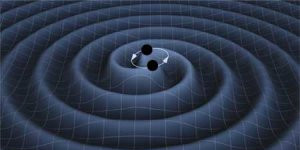
\includegraphics[width=.9\textwidth]{figuras/binary-wave_tn.jpg}
\caption{A impressão artística de ondas gravitacionais de dois buracos negros em órbita. [Imagem: T. Carnahan (NASA GSFC)]}
\label{figespaçotempo}
\end{figure}

Ondas gravitacionais são criadas por massas móveis, da mesma forma que ondas eletromagnéticas são criadas por cargas em movimento. Mas como a gravidade é a mais fraca das quatro forças fundamentais (sendo as outras o eletromagnético, o nuclear fraco e o nuclear forte), as ondas gravitacionais são extremamente pequenas, produzindo um deslocamentos da ordem de \(10^{-18}\) metros, isto é, 1000 vezes menor que o diâmetro de um próton \cite{abbott2016observation}. Ondas dessa força serão produzidas por sistemas muito massivos que passam por grandes acelerações, como dois buracos negros em órbita que estão prestes a se fundir um com o outro. Como sistemas como esses são raros, essas fontes estarão a anos-luz de distância.

Em geral, qualquer aceleração que não seja esférica ou cilíndrica simétrica produzirá uma onda gravitacional \cite{abbott2017gw170814}. Considere uma estrela que vai se transformar em supernova, esta explosão produzirá ondas gravitacionais se a massa não for ejetada de maneira esférica simétrica, embora o centro de massa possa estar na mesma posição antes e depois da explosão. Outro exemplo é uma estrela em movimento. Uma estrela perfeitamente esférica não produzirá uma onda gravitacional, mas sim uma estrela irregular \cite{abbott2017gw170817}.

As ondas gravitacionais pelas quais os detectores modernos são sensíveis estariam na faixa de frequência audível se fossem ondas sonoras. Nesse sentido, esses detectores podem ser considerados como "rádios de ondas gravitacionais" \cite{ligo2016gw151226}. Assim como as ondas de rádio não podem ser ouvidas sem um rádio para detectar as ondas de rádio e decodificar o sinal de música para os alto-falantes, ondas gravitacionais não podem ser ouvidas sem um detector para distinguir a onda gravitacional e enviar esse sinal para os alto-falantes. Toda a física que entrou na produção de uma onda gravitacional é então codificada nessa "música" para os físicos decodificarem \cite{ligo2016gw151226}. Nas descrições seguintes de ondas gravitacionais, o 'som' que eles fazem será frequentemente descrito para ilustrar as propriedades do sinal esperado. 

Existem quatro fontes principais de ondas gravitacionais causadas por diferentes tipos de movimento e mudanças na distribuição da massa: contínua , sistemas binários , ruptura e estocástica \cite{ligo2016gw151226}.

Ondas gravitacionais contínuas são produzidas por sistemas que têm uma frequência razoavelmente constante e bem definida. Exemplos disso são sistemas de estrelas binárias ou de buracos negros orbitando um ao outro ou uma única estrela girando rapidamente em torno de seu eixo com uma grande montanha ou outra irregularidade nela. Espera-se que estas fontes produzam ondas gravitacionais comparativamente fracas, uma vez que elas evoluem ao longo de períodos de tempo mais longos e são geralmente menos catastróficas do que as fontes que produzem ondas gravitacionais inspiradas ou explodidas. O som que essas ondas gravitacionais produziriam é um tom contínuo, já que a frequência da onda gravitacional é quase constante, como ilustra a Figura~\ref{figondacontinua}.

\begin{figure}[ht]
\centering
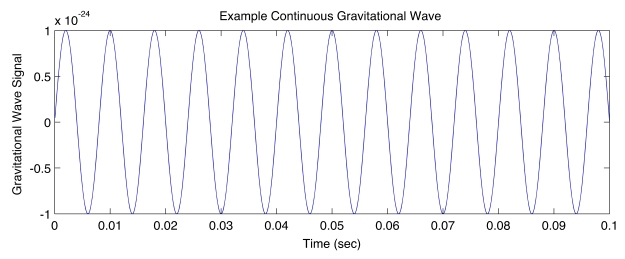
\includegraphics[width=.9\textwidth]{figuras/continuous_tn.jpg}
\caption{Um sinal de exemplo de uma fonte de onda gravitacional contínua. [Image: A. Stuver / LIGO]}
\label{figondacontinua}
\end{figure}

Ondas gravitacionais de sistemas binários são geradas durante o estágio de final de vida de sistemas binários, onde os dois objetos se fundem em um. Esses sistemas são geralmente duas estrelas de nêutrons, dois buracos negros, ou uma estrela de nêutrons e um buraco negro cujas órbitas se degradaram até o ponto em que as duas massas estão prestes a coalescer. À medida que as duas massas giram em torno uma da outra, suas distâncias orbitais diminuem e suas velocidades aumentam, muito parecido com um patinador giratório que desenha seus braços perto de seu corpo. Isso faz com que a frequência das ondas gravitacionais aumente até o momento da coalescência. O som que essas ondas gravitacionais produziriam seria um som de chilro (muito parecido com o aumento do tom rapidamente em um apito), já que a frequência orbital do sistema binário está aumentando (qualquer aumento na frequência corresponde a um aumento no tom), exemplo de onda gravitacional de sistemas binários na Figura~\ref{figondainspiral}.

\begin{figure}[ht]
\centering
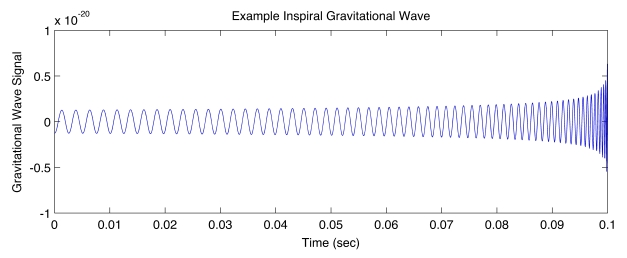
\includegraphics[width=.9\textwidth]{figuras/inspiral_tn.jpg}
\caption{Um sinal de exemplo de uma fonte de onda gravitacional de sistemas binários. [Image: A. Stuver / LIGO]}
\label{figondainspiral}
\end{figure}

As ondas gravitacionais de rupturas vêm de fontes desconhecidas ou imprevistas de curta duração, são as ondas gravitacionais que surgem à noite. Toda vez que os humanos olham para o universo com um novo conjunto de "olhos" (por exemplo, usando telescópios para observar a luz visível ou ondas de rádio, ou detectores de raios gama para ver raios gama), eles descobriram coisas que foram inesperadas e revolucionaram nossa visão. compreensão do universo. Portanto, em ondas gravitacionais de ruptura, estamos esperando o inesperado. Há hipóteses de que alguns sistemas, como supernovas ou rajadas de raios gama, podem produzir ondas gravitacionais de ruptura, mas pouco se sabe sobre os detalhes desses sistemas para antecipar a forma que essas ondas terão. A Figura~\ref{figondaruptura} ilustra como seria uma onda gravitacional de ruptura. 

\begin{figure}[ht]
\centering
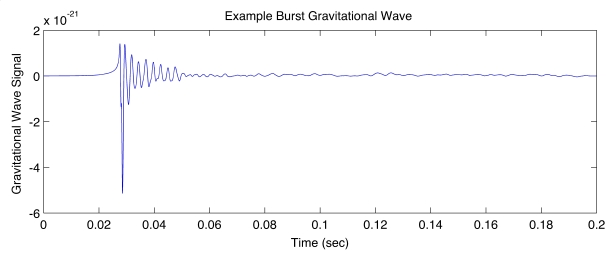
\includegraphics[width=.9\textwidth]{figuras/burst_tn.jpg}
\caption{Um sinal de exemplo de uma fonte de onda gravitacional de ruptura. [Image: A. Stuver / LIGO usando dados de C. Ott, D. Burrows e outros]}
\label{figondaruptura}
\end{figure}

Ondas gravitacionais estocásticas são as ondas gravitacionais relíquias da evolução inicial do universo. Assim como o Fundo Micro-Onda Cósmico (CMB), que provavelmente é a luz residual do Big Bang, essas ondas gravitacionais surgem de um grande número de eventos aleatórios e independentes combinados para criar um fundo de ondas gravitacionais cósmicas. Espera-se que o Big Bang seja o principal candidato para a produção dos muitos processos aleatórios necessários para gerar ondas gravitacionais estocásticas (e o CMB) e, portanto, podem conter informações sobre a origem e a história do universo. Se essas ondas gravitacionais realmente se originaram no Big Bang, essas ondas terão sido esticadas à medida que o universo se expandisse e pudessem nos contar sobre o próprio começo do universo, elas teriam sido produzidas entre aproximadamente \(10^{-36}\) a \(10^{-32}\) segundos após o Big Bang, enquanto o CMB foi produzido aproximadamente 300.000 anos após o Big Bang. O som que essas ondas gravitacionais produziriam é um ruído contínuo (muito parecido com o estático) e será o mesmo de todas as partes do céu (assim como o CMB). Fundos similares poderiam ser produzidos por uma combinação de muitas sistemas binários, rupturas ou sinais contínuos simultâneos de todo o Universo, um exemplo de onda gravitacional estocástica é apresentado na Figura~\ref{figondaestocastica}.

\begin{figure}[ht]
\centering
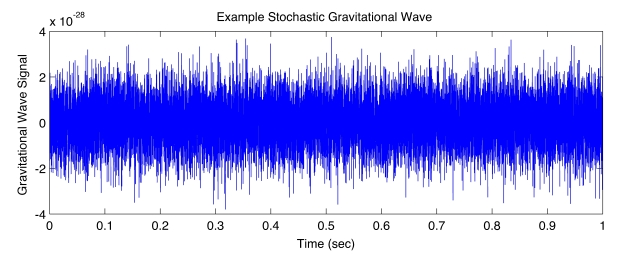
\includegraphics[width=.9\textwidth]{figuras/stochastic_tn.jpg}
\caption{Um sinal de exemplo de uma fonte de onda gravitacional estocástica. [Imagem: A. Stuver / LIGO]}
\label{figondaestocastica}
\end{figure}

As ondas gravitacionais existem em dois estados de polarização normalmente designados por + e x Figura~\ref{figpolarization}. A polarização fornece, entre outras coisas, informação sobre a inclinação do plano orbital de um sistema binário em relação ao observador. Quando a linha de observação é paralela ao plano orbital do sistema, cada uma das componentes aparenta mover-se numa linha reta e é neste caso possível mostrar que a polarização das ondas gravitacionais emitidas será linear. Se, pelo contrário, a linha de observação for normal ao plano orbital, o movimento das estrelas será circular e a polarização observada será também circular. Entre estes dois casos limite existe uma gama de valores possível para a inclinação do plano orbital que pode em princípio ser deduzida através da polarização do sinal observado.

\begin{figure}[ht]
\centering
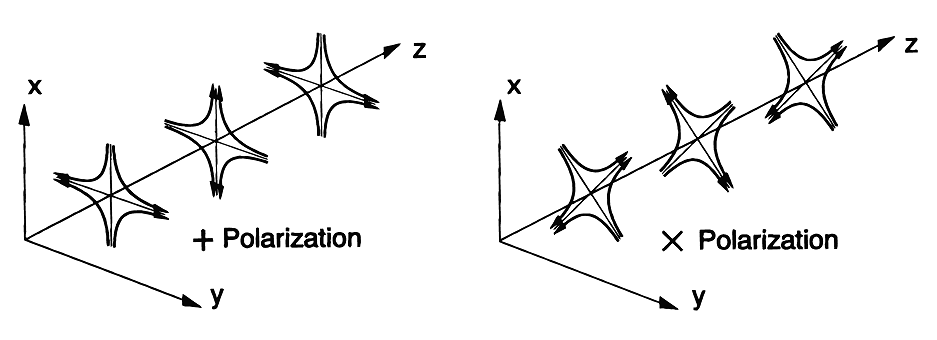
\includegraphics[width=.9\textwidth]{figuras/polarization.png}
\caption{Modos de polarização das ondas gravitacionais h + e h x propagando-se na direção z. [Imagem: \cite{centrella2010black}]}
\label{figpolarization}
\end{figure}

\section{Redes Neurais Artificiais}
O cérebro humano é considerado o mais fascinante processador existente. Ele é composto por aproximadamente 10 bilhões de neurônios, que são responsáveis por todas as funções e movimentos do nosso organismo. Os neurônios estão conectados uns aos outros através de sinapses, e juntos formam uma grande rede, denominada Rede Neural, que proporciona uma fabulosa capacidade de processamento e armazenamento de informação, Figura~\ref{figneuronios}.

\begin{figure}[ht]
\centering
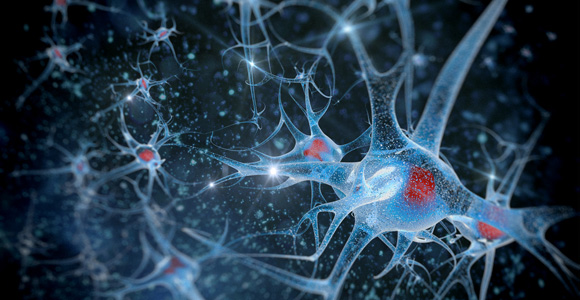
\includegraphics[width=1\textwidth]{figuras/axons.jpg}
\caption{Rede neural humana: o melhor processador de informações existente. [Imagem: \href{ https://neurogestion.wordpress.com}{ https://neurogestion.wordpress.com}]}
\label{figneuronios}
\end{figure}

Há algumas décadas, surgiu a ideia de modelar, computacionalmente, as conexões neurais do cérebro humano, com intuito de emergir comportamentos inteligentes em máquinas. Neste contexto, surgiu as Redes Neurais Artificiais (RNA's), inspiradas na própria natureza das redes de neurônios cerebrais e sinapses biológicas.

O trabalho em RNA's, comumente chamadas de “redes neurais” (RN), foi motivado desde o início pelo reconhecimento de que o cérebro humano computa de uma forma totalmente diferente do computador digital convencional. O cérebro é um computador altamente complexo, não linear e paralelo \cite{haykin2009neural}.

Uma rede neural artificial é um um sistema de processamento paralelo de informações constituído pela interconexão de unidades básicas de processamento, denominadas neurônios artificiais, que tem a propensão natural para armazenar conhecimento experimental e torná-lo disponível para o uso \cite{haykin2009neural}. Todo conhecimento adquirido pela rede se da através de um algoritmo de aprendizagem, cuja função é modificar os pesos de conexões entre os neurônios da rede, conhecidos como pesos sinápticos, de forma ordenada a fim de alcançar o mapeamento desejado.

O neurônio artificial é a menor unidade de processamento de uma rede neural, que recebe sinais de entrada e produzem sinais de saída. O modelo de neurônio mais utilizado é o perceptron, representado na equação~\ref{eq1}, que é composto por: m entradas (\(x_1, \ldots ,x_m\)), m pesos sinápticos (\(w_1, \ldots , w_m\)), uma variável de deslocamento linear \(b\) (do inglês: bias) e uma saída \(y\).

\begin{equation} \label{eq1}
\begin{split}
y = \theta(\sum_{i=1}^{m} x_i w_i + b)
\end{split}
\end{equation}

A função \(\theta\) é conhecida como função de ativação ou função de transferência. Dentre as funções de ativação mais utilizadas estão a sigmoide e a tangente hiperbólica, definidas pelas equações abaixo, respectivamente:

\begin{equation} \label{eq2}
\begin{split}
\theta(u) & = \frac{1}{1+ e^{-au}}\\
\theta(u) & = \frac{e^u - e^{-u}}{e^u + e^{-u}}
\end{split}
\end{equation}

A arquitetura de uma rede neural está relacionada com a maneira pela qual os neurônios da mesma estão organizados. Para isso, a rede é dividida em três tipos de camadas: a de entrada, a escondida e a de saída. As camadas de entrada e saída são intuitivas e representam o número de entradas e saídas do problema em questão. Já a escondida é a camada que fará a maior parte do processo de aprendizagem da rede. Normalmente uma rede neural possui uma camada de entrada, uma camada de saída e \(k\) camadas escondidas, no qual \(k\) é definido empiricamente e varia de acordo com o problema. Com isso forma-se uma rede de múltiplas camadas.

Redes neurais do tipo Feedforward (em português costumam traduzir como alimentação direta ou avante) são redes de múltiplas camadas no qual a informação só propaga em um sentido. No caso, os sinais provenientes dos neurônios de uma camada só podem estimular os neurônios da camada seguinte, não existindo realimentação. A Figura~\ref{figredeFeedforward} mostra uma rede neural de múltiplas camadas do tipo Feedforward, com uma camada de entrada, com m entradas, \(k\) camadas escondidas com \(j\) neurônios e uma camada de saída com \(n\) saídas.

\begin{figure}[ht]
\centering
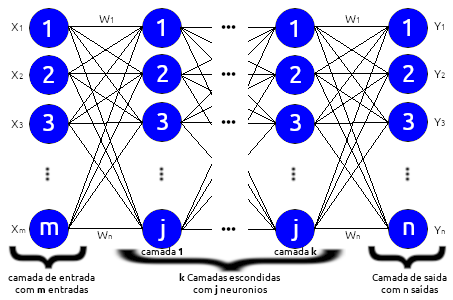
\includegraphics[width=1\textwidth]{figuras/rede_neural_Feedforward.png}
\caption{Exemplo de rede neural artificial do tipo feedforward. [Imagem: Elaborada pelo autor]}
\label{figredeFeedforward}
\end{figure}

Após projetada a arquitetura da rede (determinar número de entradas, saídas, camadas escondidas e número de neurônios), é necessário um algoritmo de treinamento para realizar a aprendizagem da mesma. No processo de treinamento a rede ‘aprende’ através de exemplos que relacionam as entradas e saídas do problema a ser solucionado. Essa abordagem é conhecida como aprendizado supervisionado. Dentre os algoritmos conhecidos, para solucionar esse tipo de problema, o mais utilizado é o backpropagation \cite{rumelhart1986learning}. A ideia do algoritmo é estimar os valores dos pesos e bias minimizando o erro entre a entrada e a saída desejada usando o gradiente descendente. O erro \(E\) cometido pela rede é calculado por:

\begin{equation} \label{eq3}
\begin{split}
E = \frac{1}{2} \sum_{i=1}^{p} \sum_{j=1}^{n} (d_{j}^{i} - y_{j}^{i})^2
\end{split}
\end{equation}

no qual, \(p\) é o número exemplos a ser utilizados no treinamento, n é o número de saídas da rede e, finalmente, \(d\) e \(y\) são as saídas desejadas e obtidas, respectivamente, para a entrada em curso.
A regra de atualização de cada peso sináptico da rede é calculado pela seguinte equação:

\begin{equation} \label{eq4}
\begin{split}
W = W + \Delta W \therefore \Delta W = \alpha\frac{\partial E}{\partial W}
\end{split}
\end{equation}

onde, \(\alpha\) é conhecido como taxa de aprendizado, que, resumidamente, indica o ‘tamanho do passo’ do gradiente rumo a minimização. O sinal negativo indica a busca por uma alteração no peso que reduza \(E\).

\section{Extreme Learning Machine}

Extreme Learning Machine (ELM, ou em português, máquina de aprendizado extremo), algoritmo proposto por Huang \cite{1380068, HUANG2006489} e que nada mais é do que uma rede neural artificial (RNA) de apenas uma camada oculta. O princípio de funcionamento da ELM é o mesmo de uma RNA, todavia a metodologia de treinamento de uma ELM não é baseada em gradiente descendente. Com isso o algoritmo escapa das principais deficiências do backpropagation: convergência lenta e convergência para mínimos locais. Segundo \cite{HUANG2006489} o treinamento de uma ELM pode ser milhares de vezes mais rápido do que o treinamento via backpropagation. A Figura~\ref{figredeextreme} ilustra a arquitetura de uma ELM, muito semelhante com a arquitetura de uma RNA, descrita anteriormente, porém com \(k = 1\), ou seja, temos apenas uma camada oculta.

\begin{figure}[ht]
\centering
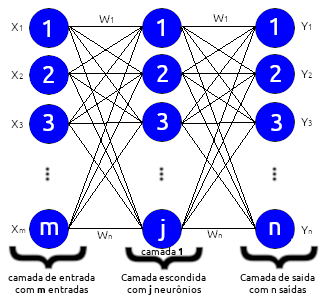
\includegraphics[width=1\textwidth,height=.75\textwidth]{figuras/extreme_learning_machine.png}
\caption{arquitetura de uma rede neural artificial. A ELM utiliza apenas uma camada oculta, portanto, k = 1. [Imagem: Elaborada pelo autor]}
\label{figredeextreme}
\end{figure}

O vetor \(\mathbf{X}\) é a entrada da rede. Os pesos de conexão da camada de entrada são alocados em uma matriz denominada \(\mathbf{w}\) e já os da camada oculta em uma matriz denominada \(\boldsymbol{\beta}\). Para facilitar e agilizar os cálculos, os bias dos neurônios da camada oculta também são alocados na última linha de \(\mathbf{w}\), e os bias da camada de saída não são utilizados na ELM. A modelagem matricial do ELM é descrita na Equação~\eqref{eq5}:

\begin{subequations} \label{eq5}
\begin{align}
        \boldsymbol{X} &= \begin{bmatrix}
                x_{1},      & \dots ,     & x_{m},    & 1
            \end{bmatrix}, \\
        \boldsymbol{W} &= \begin{bmatrix}
                w_{11}      & \dots     & w_{1j} \\
                \vdots      & \ddots    & \vdots \\
                w_{m1}      & \dots     & w_{mj} \\
                b_{1}      & \dots     & b_{j} \\
            \end{bmatrix}, \\
        \boldsymbol{\beta}. &= \begin{bmatrix}
                \beta_{11}      & \dots     & \beta_{1n} \\
                \vdots      & \ddots    & \vdots \\
                \beta_{j1}      & \dots     & \beta_{jn}
            \end{bmatrix}, \\
            \boldsymbol{Y} &= \begin{bmatrix}
                y_{1},      & \dots ,     & y_{n}
            \end{bmatrix}
\end{align}
\end{subequations}

onde \(m\) é o número de neurônios de entradas, \(j\) é o número de neurônios na camada oculta e \(n\) é o número de neurônios de saída da rede.

\subsection{Treinamento}

O treinamento da ELM é realizado de maneira analítica, diferentemente da abordagem iterativa do backpropagation. A matriz \(\mathbf{w}\) é gerada de maneira aleatória e não é alterada até o fim do algoritmo. Portanto, o objetivo do treinamento da ELM é encontrar a matriz de pesos \(\boldsymbol{\beta}\), baseado na matriz de saída \(\mathbf{y}\) e na matriz de pesos aleatórios \(\mathbf{w}\), por meio da resolução de um sistema linear. Para isso, o primeiro passo é determinar a matriz \(\mathbf{H}\) como mostra a Equação~\eqref{eq6}.

\begin{equation} \label{eq6}
\begin{split}
\mathbf{H}^i = [x_{1}^{i}, \dots , x_{m}^{i},1]                             \begin{bmatrix}
                w_{11}      & \dots     & w_{1n} \\
                \vdots      & \ddots    & \vdots \\
                w_{m1}      & \dots     & w_{mj} \\
                b_{1}      & \dots     & b_{j}
            \end{bmatrix} \Rightarrow \mathbf{H} = \begin{bmatrix}
                f(H^1) \\
                f(H^2) \\
                \vdots \\
                f(H^S)
            \end{bmatrix}_{S \times j}
\end{split}
\end{equation}

onde a função \(f(.)\) é a função de transferência (pode ser uma sigmoide, por exemplo) da camada e \(i =\) \{\(1, \dots , S\)\}, sendo \(\mathbf{S}\) o número de amostras do conjunto de treinamento. Portanto, a matriz \(\mathbf{H}\) armazena o resultado de todos os neurônios da camada oculta obtidos a partir da multiplicação entre \(\mathbf{X}\) e \(\mathbf{W}\). Uma vez determinada a matriz \(\mathbf{H}\), para se obter os pesos da matriz \(\boldsymbol{\beta}\) deve ser solucionado o sistema linear da Equação~\eqref{eq7}.

\begin{equation} \label{eq7}
\begin{split}
\mathbf{H} \boldsymbol{\beta} = \mathbf{Y} \rightarrow \boldsymbol{\beta} = \mathbf{H}^\dagger \mathbf{Y} 
\end{split}
\end{equation}

onde \(\mathbf{H}^{\dagger}\) é a inversa generalizada de Moore–Penrose \cite{serre2010matrices} da matriz \(\mathbf{H}\). Caso fosse utilizado a inversa padrão, o algoritmos seria limitado a problemas que essa inversa existisse. A inversa generalizada ‘afrouxa’ algumas exigências da inversa tradicional, como por exemplo, a matriz não precisa ser quadrada.

Devido ao fato do treinamento da ELM ser executado de forma analítica, o mesmo é realizado de maneira mais rápida do que um método iterativo \cite{HUANG2006489}. Todavia a abordagem possui suas fraquezas. A primeira delas é relacionada a inicialização aleatória dos pesos da matriz \(\mathbf{W}\). Pode ocorrer dos valores obtidos para \(\mathbf{W}\) desencadear, ao fim do processo, em uma matriz \(\boldsymbol{\beta}\) que proporcione um resultado final ruim. Por conta disso, existem trabalhos que visam otimizar a escolha dos valores de \(\mathbf{W}\) por meio de algoritmos evolutivos \cite{HAN201387}, por exemplo. Outra fraqueza é o fato do algoritmo trabalhar com a inversa generalizada da matriz \(\mathbf{H}\). Caso a rede possua muitas amostras e muitos neurônios na camada oculta, obter a inversa generalizada de \(\mathbf{H}\) pode demandar bastante recurso computacional.